\chapter{Search for di-Higgs Production in the \texorpdfstring{$\gamma\gamma b\bar{b}$}{yybb} Channel}
\section{Analysis Overview}

Previous results were presented with an integrated luminosity of 36.1 fb$^{-1}$ representing ATLAS dataset in 2015 and 2016 \cite{HIGG-2016-15}, and were consistent with Standard Model expectations. The non-resonant analysis set an observed (expected) 95\% CL upper limit on the $HH$ cross-section of 0.73 (0.93) pb, corresponding to 22 (28) times the SM prediction. This Higgs trilinear coupling is constrained between $-8.2 < \kappa_\lambda < 13.2$ at 95\% CL ($-8.3 < \kappa_\lambda < 13.2$ expected). The resonant analysis presented within the context of a narrow width scalar coupling to the di-Higgs system as a function of $m_X$. The observed (expected) limits are between 1.1 pb (0.9 pb) and 0.12 pb (0.15 pb) over the range of $\unit{260}{\GeV} < m_X < \unit{1000}{\GeV}$.

\section{Data and Simulated Samples}


\subsection{Data}

The analysis presented uses $pp$ collision data recorded by the ATLAS experiment at the LHC during ``Run 2,'' which ran from 2015 through 2018. After detector and data quality requirements, the total collected data corresponds to 139 \ifb. The loose diphoton trigger is used for this search, \texttt{HLT\_g35\_loose\_g25\_loose}, which triggers on diphoton events where the leading (subleading) photon \pt is greater than 35\% (25\%) the diphoton invariant mass.

\subsection{Signal Samples}

This analysis searches for both non-resonant and resonant di-Higgs production, considering signal contributions from the ggF and VBF production modes.

\subsubsection{Non-resonant VBF HH Samples}

The signal MC samples for VBF $HH$ production are generated at LO using \MGMCatNLO 2.6.0, using cards presented in \cite{vbfhh}. The process generated is $pp \rightarrow HHqq$. The dominant production in this sample is VBF $HH$ production, but contains contributions from $VHH$  hadronic and Higgsstrahlung production. The NNPDF 2.3 LO PDF set \cite{NNPDF} is used in the matrix element, interfaced to \HERWIG 7.0.4 using the H7-UE-MMHT tune for underlying events and the H7-MMHT2014LO tune for parton shower and hadronization.

Samples have been produced for the various coupling values shown in Table \ref{tab:vbf-coupling-samples}. The values of $\kappa_\lambda$,$c_{2V}$, and $c_{v}$ are all 1 in the SM. The values selected for production aim to vary each coupling value enough that interpolation may be performed, and one value was produced near where limits could be expected to be set ($\kappa_\lambda = 10$ and $c_{2V}=4$).

\begin{table}[htbp]
    \centering
    \begin{tabular}{c|c|c}
        $\kappa_\lambda$ & $c_{2V}$ & $c_{v}$ \\
        \hline
        1 & 0 & 0.5 \\
        1 & 1 & 0.5 \\
        0 & 0 & 1 \\
        1 & 0 & 1 \\
        1 & 0.5 & 1 \\
        1 & 0 & 0.5 \\
        1 & 1 & 1 \\
        1 & 1.5 & 1 \\
        1 & 2 & 1 \\
        1 & 4 & 1 \\
        0 & 1 & 1 \\
        2 & 1 & 1 \\
        10 & 1 & 1 \\
        1 & 1 & 1.5
    \end{tabular}
    \caption{Grid of coupling values used in production of VBF $HH$ samples.}
    \label{tab:vbf-coupling-samples}
\end{table}

Relevant distributions for validation of these samples can be seen in Figure \ref{fig:vbf-mc-validation}. Plots are shown at parton level, with a basic jet selection applied to isolate the VBF jets similar to that done at reconstruction level. Jets are considered if they have $\pt > 25$, then the $m_{bb}$ pair is selected as the two jets with $m_{bb}$ closest to 125 \GeV. The VBF jets are selected as the highest $m_{jj}$ pair after removing jets used in the $m_{bb}$ pairing. Additional detail on the validation for these samples is outlined in Ref. \cite{mc-validation}.

\begin{figure}[htbp]
    \centering
    \subfloat{
      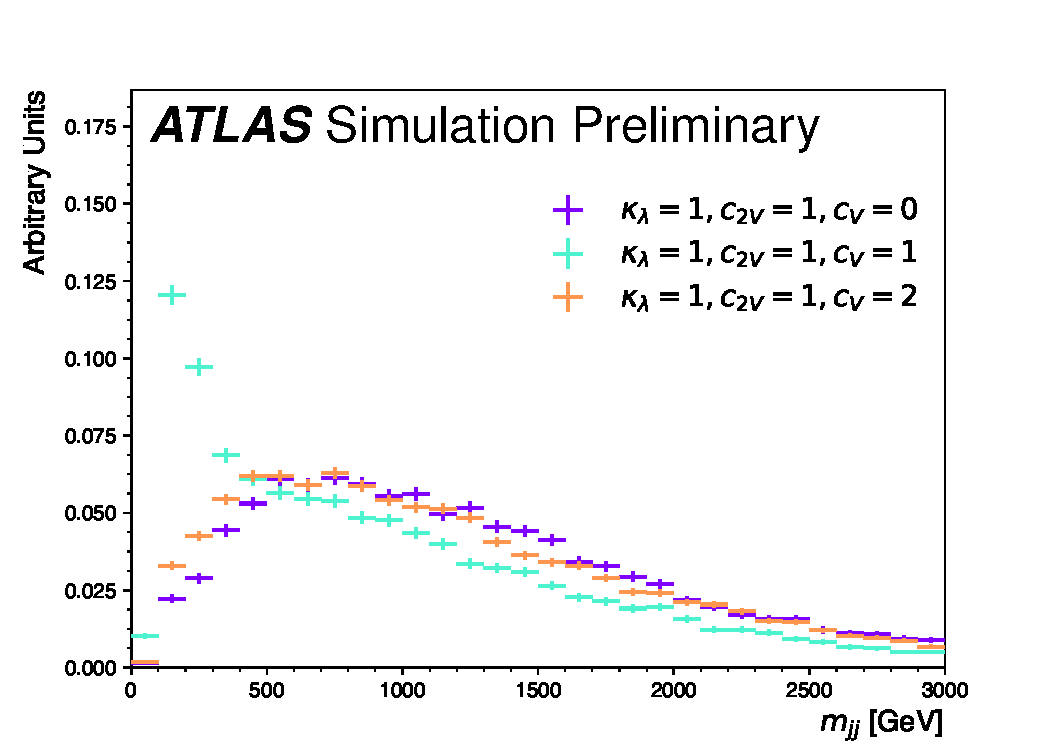
\includegraphics[width=0.33\textwidth]{chapters/chapter5_yybb/images/mc_samples/m_jj_cv.pdf}
    }
    \subfloat{
      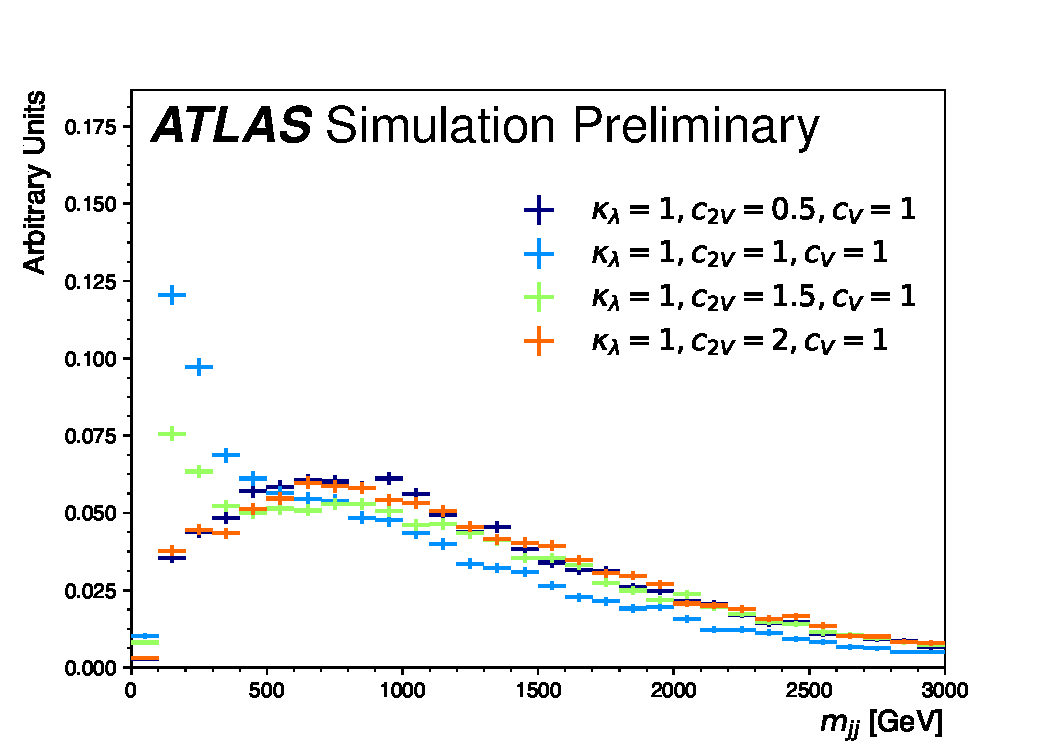
\includegraphics[width= 0.33\textwidth]{chapters/chapter5_yybb/images/mc_samples/m_jj_cvv.pdf}
    }
    \subfloat{
      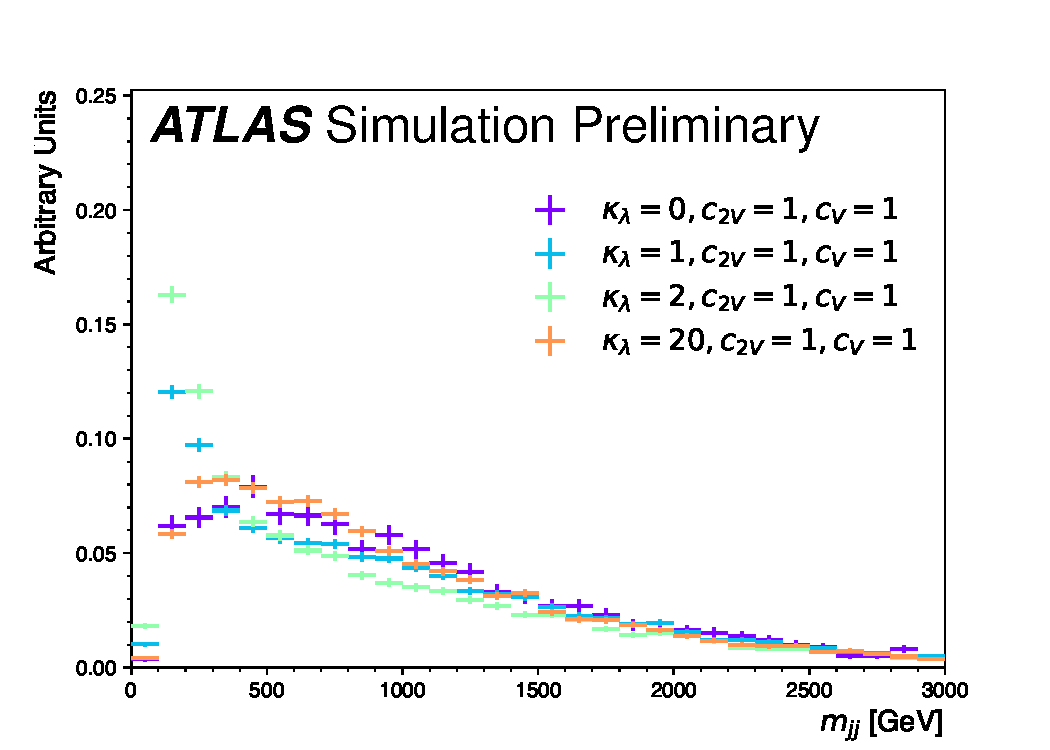
\includegraphics[width= 0.33\textwidth]{chapters/chapter5_yybb/images/mc_samples/m_jj_klambda.pdf}

    }       

    \subfloat{
        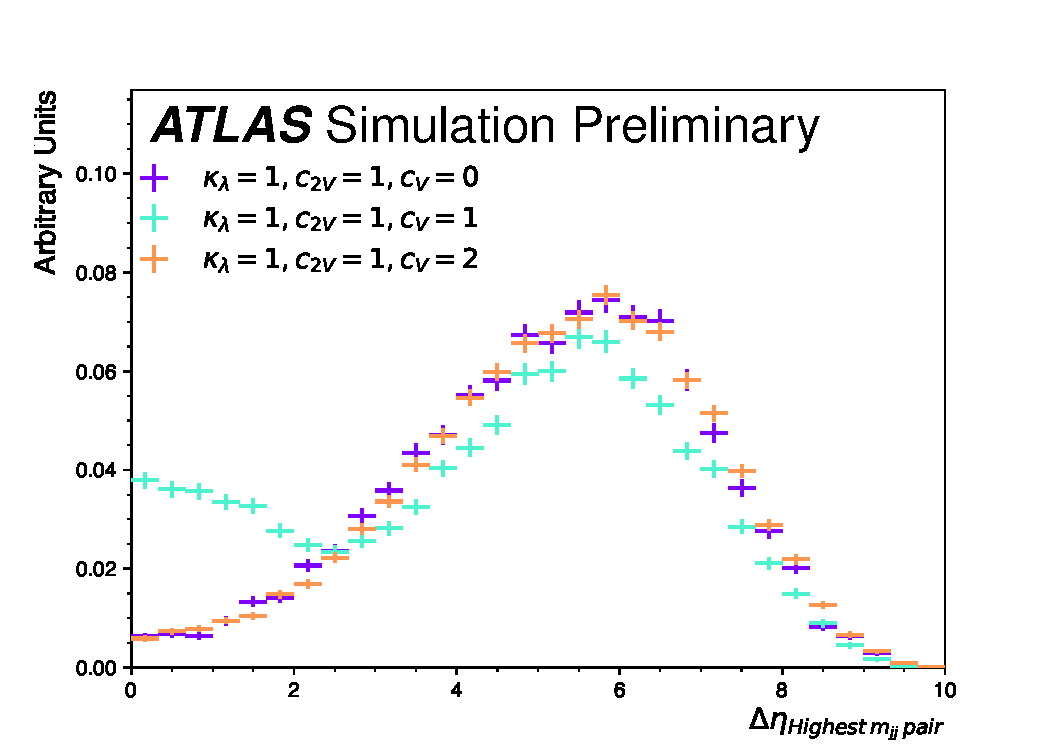
\includegraphics[width=0.33\textwidth]{chapters/chapter5_yybb/images/mc_samples/jj_deta_cv.pdf}
      }
      \subfloat{
        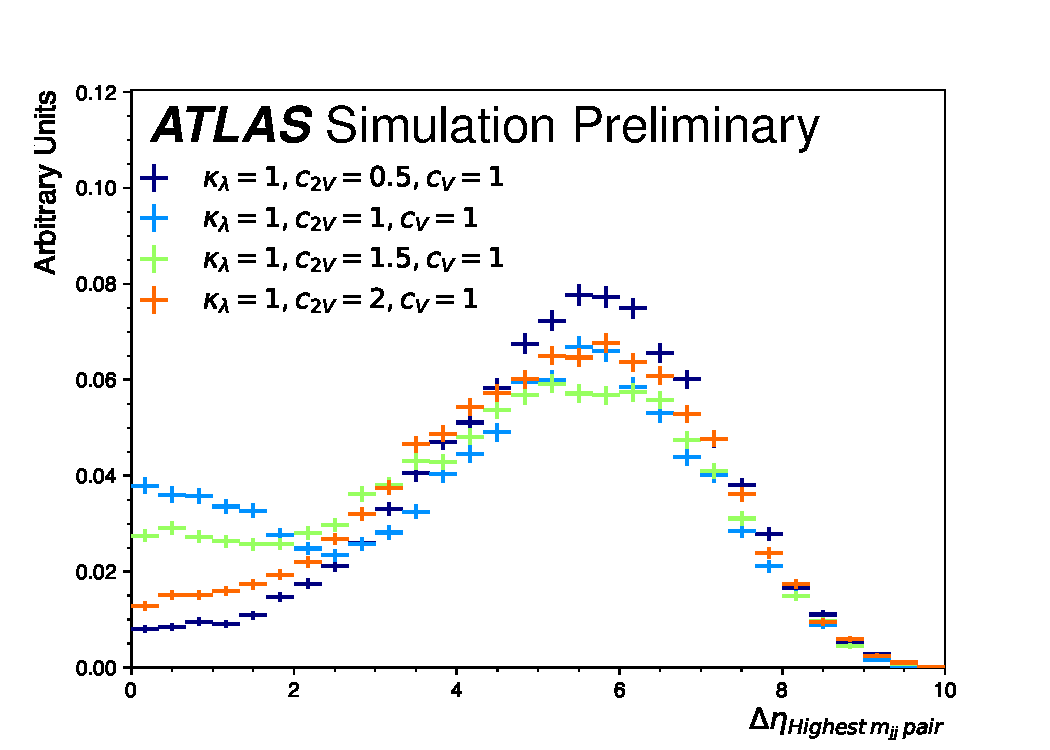
\includegraphics[width= 0.33\textwidth]{chapters/chapter5_yybb/images/mc_samples/jj_deta_cvv.pdf}
      }
      \subfloat{
        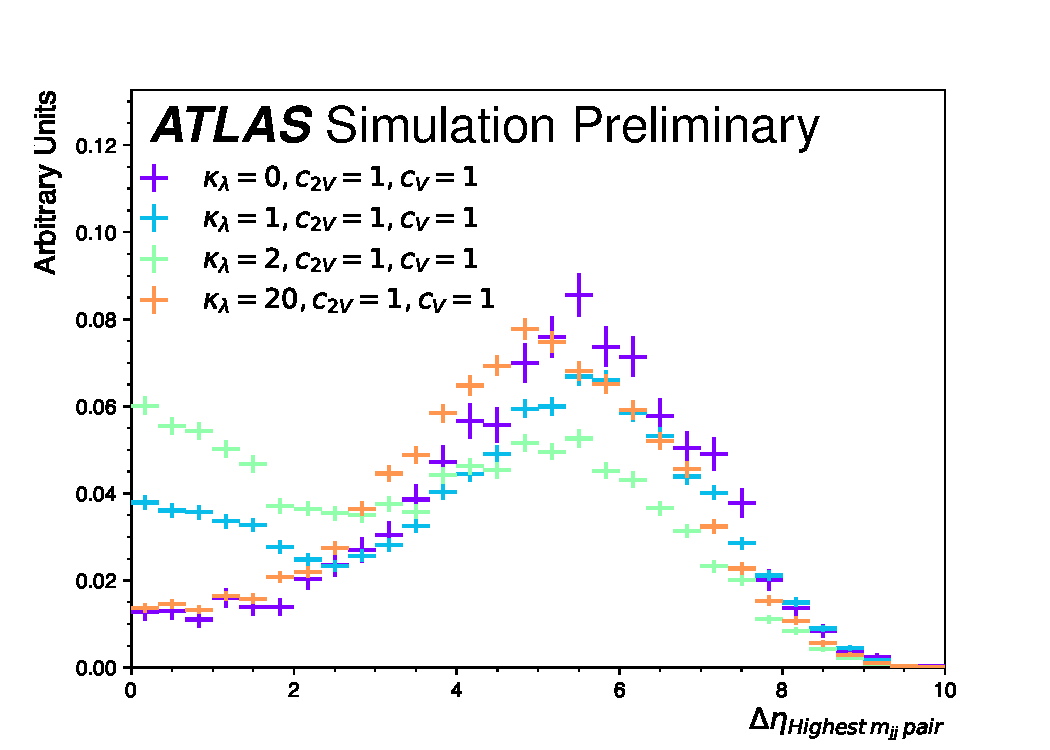
\includegraphics[width= 0.33\textwidth]{chapters/chapter5_yybb/images/mc_samples/jj_deta_klambda.pdf}
    }    

    \caption{Validation plots at parton level for the VBF $HH$ signal sample. The highest $m_{jj}$ pair is selected as a proxy for the VBF jets. The top row shows the invariant mass distribution of this system, the bottom depicts the $\Delta \eta$ between these jets. Left to right, these plots vary the $c_V$, $c_{2V}$, and $\kappa_\lambda$ strength. The peak at low $m_{jj}$ values and shoulder at low $\Delta \eta$ is a product of the $VHH$ hadronic and Higgsstrahlung contributions in the samples.}
    \label{fig:vbf-mc-validation}
\end{figure}

\section{Object Definition}
\section{Event Selection}
\section{Modeling}
\subsection{Signal Modeling}
\subsection{Background Modeling}
\section{Systematic Uncertainties}
\section{Results}
\subsection{Limits on Non-Resonant Production}
\subsection{Limits on Resonant Production}
\subsection{Limits on the Trilinear Higgs Coupling}
\section{Searches for Vector Boson Fusion HH Production}
\subsection{Simulated Samples}
\subsection{Event Selection}
\subsection{Analysis Improvement}
